% *******************************************************************************
% * Copyright (c) 2007 by Elexis
% * All rights reserved. This document and the accompanying materials
% * are made available under the terms of the Eclipse Public License v1.0
% * which accompanies this distribution, and is available at
% * http://www.eclipse.org/legal/epl-v10.html
% *
% * Contributors:
% *    G. Weirich - initial implementation
% *
% *  $Id: konsviews.tex 4902 2009-01-03 10:47:34Z rgw_ch $
% *******************************************************************************
% !Mode:: "TeX:UTF-8" (encoding info for WinEdt)


\section{'Views' en rapport avec les consultations}



\subsection{Cas}
Cette view (Fig. \ref{fig:faelle2} létabli une liste de tout les cas du patient actuellement sélectionné. \index{Liste des cas}
\begin{wrapfigure}{l}{6.8cm}
  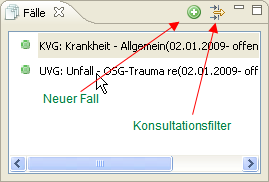
\includegraphics{images/faelleview}
  \caption{Fälle - View}
  \label{fig:faelle2}
\end{wrapfigure}

Le symbole qui se trouve à gauche de la désignation du cas indique si toutes les données nécessaires ont été rassemblées pour que la facturation puisse être faite : S'il est vert, l'établissement de facture devrait être possible, s'il est rouge, manque encore une ou plusieurs données.


\textit{Quelles} indications minimales sont nécessaires, dépend du système de facturation. Ainsi, pour les cas qui sont facturés selon la LAMal,l'indication d'un destinataire de la facture, d'un 	assureur et du numéro d'assurance est nécessaire. Les cas qui sont comptabilisés selon la LAA nécessitent un numéro de cas. Pour des factures en privé un destinataire de la facture devra au moins être indiqué.

\medskip

\index{filtrer!consultations}
\label{filter:fall}
Un clic sur le symbole de filtre dans l'entête de la 'View' a pour conséquence qu'il n'y a plus que les consultations dans la liste de consultation (cf \ref{view:konsultationen}) qui font partie du cas choisi actuellement. Si on choisi un autre cas, la liste est de nouveau filtrée. Cliquez encore une fois sur le symbole de filtre pour éteindre le filtre.

Le clic droit sur un cas ouvre son menu de contexte. Celui-ci contient les points
suivants :

\begin{itemize}
  \item {Supprimer un cas}. Ceci n'est possible, que si vous avez les droits nécessaires, et si plus aucune consultation n'existe .
  \item {Modifier un cas }. Ceci ouvre une autre 'View', dans laquelle les détails pour le cas actuellement séléctionné peuvent être introduits.
  \item {Réouverture du cas}. Ceci permet de réactiver un cas déjà fermé. \footnote{Un cas est fermé si une date de fin a été introduite. On ne peut plus ajouter une consultation à un cas fermé.}
  \item {Créer une facture}. Par ceci, une facture peut être produite qui concerne toutes les consultations non comptabilisées du cas actuel et du mandant actuel. Il s'agit d'un \glqq raccourci\grqq{} du procédé normale de l'établissement de facture qui convient surtout pour l'établissement immédiat de différentes consultations ou prestations.
\end{itemize}


\clubpenalty=5000

\subsection{Cas et consultations}
 %\usepackage{graphics} is needed for \includegraphics
\begin{wrapfigure}{l}{7cm}
  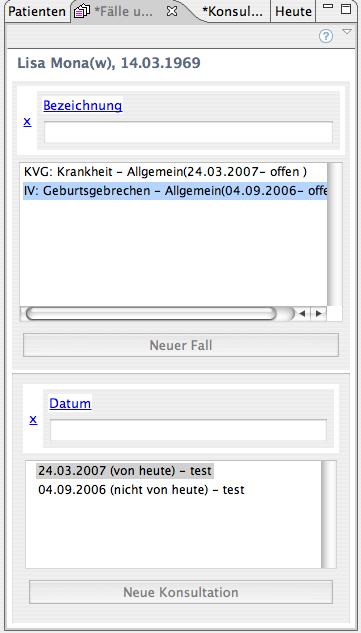
\includegraphics[width=7cm]{images/fallkonsview}
  \caption{Fälle und Kons}
  \label{fig:fallkons}
\end{wrapfigure}
Cette View (Fig. \ref{fig:fallkons} montre une liste synoptique des cas et des consultations correspondantes (seulement titres sans textes). Si on choisi dans le secteur supérieur un cas en cliquant dessus, les consultations correspondantes de ce cas sont indiquées dans le secteur inférieur.
Si on clique sur une consultation elle sera affichée dans la 'View' - consultation.
(cf page \ref{konsview} s. \pageref{konsview})

Pour établir un nouveau cas introduisez un titre pour ce cas et cliquez sur \textit{nouveau cas}. Pour une nouvelle consultation choisissez le cas concerné et cliquez sur  \textit{nouvelle consultation}

\medskip

Remarque : Vous avez constaté que cette 'View' et la View 'Cas' traité antérieurement sont jusqu'à un certain point redondantes. C'est ainsi. Vous pouvez préférer des 'Views' séparés pour les 'Cas' et les 'Consultations' ou favoriser une seule 'View' qui contient les deux. En général, vous n'appliquerez pas les deux concepts en même temps, mais celui qui vous convient mieux - Elexis vous laisse le choix.


\clearpage

\subsection{Historique des Consultations}
\label{view:konsultationen}
\begin{wrapfigure}{L}{7.5cm}
  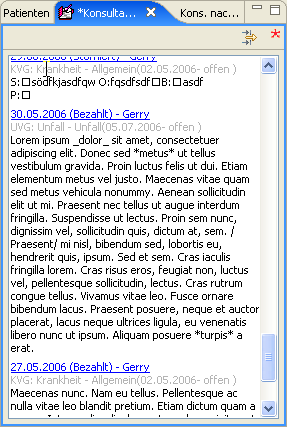
\includegraphics{images/konslisteview}
  \caption{Konsultationsliste}
  \label{fig:konslisteview}
\end{wrapfigure}

Ceci est une énumération de toutes les consultations précédentes du patient actuellement sélectionné, indépendamment du cas respectif.
\index{liste des consultations} Pour chaque consultation le texte est affiché sans formatages. (cf Fig.\ref{fig:konslisteview}).\\
En cliquant sur le titre (bleu) d'une consultation vous choisissez cette consultation dans la 'View Consultation' (cf page \pageref{konsview}).

En cliquant sur le symbole du filtre à droite en haut vous ouvrez la fenêtre du dialogue du filtre (cf Fig. \ref{fig:konsfilter}).
\index{Filtre consultations} C'est ici que vous pouvez introduire les critères selon lesquels les consultations devraient être filtrées avant d'être affichées (que les consultations qui correspondent aux conditions du filtre soient affichées).
Dans le champ supérieur vous pouvez indiquer si seulement des consultations d'un certain cas ou si tous les cas doivent être affichés. Dans le champ  inférieur, vous pouvez suggérer les critères de recherche qui doivent exister dans le texte de la consultation. Plusieurs termes de recherche peuvent ainsi être liés avec AND, OR, NOT,AND NOT et OR NOT.

Par exemple si on introduit \glqq Lorem AND NOT ipsum\grqq{} on ne trouve que les consultations dont le texte contient  \glqq Lorem\grqq, mais pas \glqq ipsum\grqq{}.

Tout en bas vous pouvez enfin encore indiquer si l'écriture majuscule/minuscule doit être considérée, ou si des critères de recherche doivent être considérés comme des termes fixes. Une explication précise de ce thème irait ici trop loin ; à ce sujet vous pouvez trouver beaucoup de littérature en utilisant les mots de recherche \glqq Regular
Expression\grqq{}ou \glqq Pattern Matching\grqq{}. Cette technique permet de décrire le critère de recherche avec différents caractères de remplacement. Ainsi permet p. ex.\glqq M[ae][iy]e?r\grqq{} de chercher tous les Meiers, Mayrs etc. donc toutes les formes d'écritures.

\medskip

Remarque : 
Filtrer l'historique par cette procédure peut durer quelques secondes, puisque le texte de chaque consultation doit être fouillé complètement. Si on veut filtrer seulement d'après des cas ou des problèmes, le filtre par cas correspondant  (cf \pageref{filter:fall}) ou le filtre de liste de problème  (cf \pageref{filter:problemliste})est en général plus efficace.

\begin{figure}[ht]
\begin{center}
  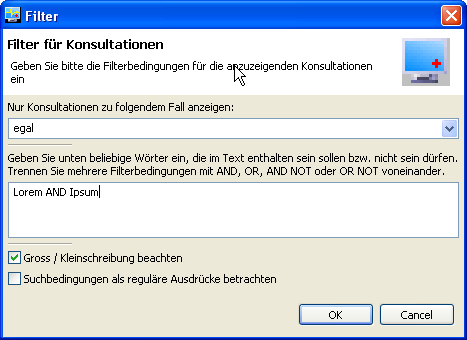
\includegraphics{images/filterdialog}
  \caption{Filterdialog}
  \label{fig:konsfilter}
\end{center}
\end{figure}


\subsection{Consultation}
 \label{konsview}
Aperçu détaillé d'une saisie de consultation(cf Fig. \ref{fig:konsdetail}).
\begin{figure}[ht]
  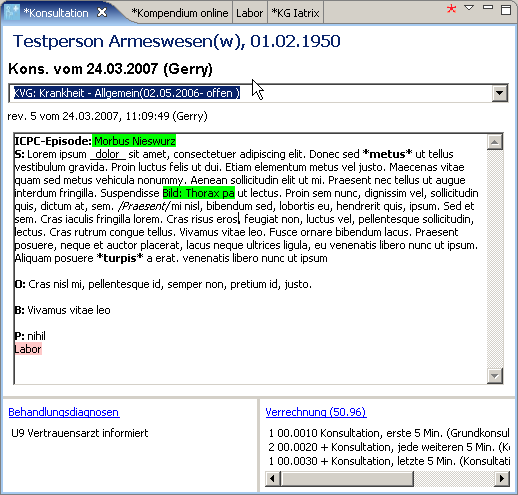
\includegraphics{images/konsview}
  \caption{Konsultation: Detail}
  \label{fig:konsdetail}
\end{figure}

Vous trouvez dans la zone de texte les possibilités supplémentaires suivantes :
\begin{description}
\item[Makros]
Ecrivez un texte quelconque, marquez-le avec la touche gauche de la souris, cliquez ensuite avec la touche droite de la souris et choisissez  'comme macro…' . Donnez un nom arbitraire à la macro. Si vous tapez à l'avenir le nom de la macro suivi d'un \# le texte prédéfini de la macro est introduit dans le texte.

\item[Introduire des prestations]
Si vous tapez le nom d'un bloc de prestation suivi d'un \#, ce bloc est comptabilisé comme si vous l'aviez tiré avec la souris dans au champ de facturation.


\item[Commandes du texte ]
Il est possible d'introduire quelques commandes simples du texte:
Un mot au début d'une ligne qui est suivi d'un deux-points se présente en caractères gras, la même chose est le cas pour mot entre deux  *. Un mot entre deux  / est écrit en italique.
\end{description}


\subsection{Certificat d'incapacité de travail}
Cette 'View' sert à fixer une incapacité de travail . (Fig. \ref{fig:auf})
\index{Certificat} \index{Certificat d'incapacité de travail}.
\begin{figure}
  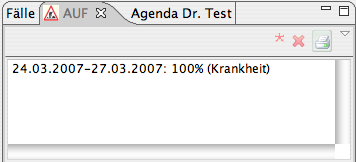
\includegraphics{images/aufview}
  \caption{AUF-View}
  \label{fig:auf}
\end{figure}
Une incapacité de travail se réfère toujours à un cas spécifique. Si aucun cas est marqué, vous serez d'abord invité d'en marquer un.

Si vous cliquez sur le symbole  \glqq nouveau\grqq (bouton vert avec un plus blanc), il apparaît une fenêtre dans laquelle vous pouvez fixer le début et la fin de l'arrêt de travail de même que le pourcentage de l'incapacité.
En cliquant sur le symbole de \glqq l'imprimante \grqq, une 'View'-Texte s'ouvre où vous pouvez effectuer encore manuellement des adaptations du texte du certificat avant de l'imprimer ou de le faxer.

\subsection{Ordonnances}
Dans cette 'View' les ordonnances seront enregistrées.  \index{ordonnance} Cliquez sur le symbole\glqq nouveau\grqq
(bouton vert avec un plus vert) pour créer une nouvelle ordonnance avec la date actuelle. Tirez les articles (médicaments) par 'Drag and Drop' d'une liste d'article ou de la 'View de médication à long terme' dans cette ordonnance. En cliquant sur le symbole \glqq imprimante\grqq vous ouvrez une 'texte-View' dans laquelle vous pouvez encore faire des modifications manuelles avant d'envoyer l'ordonnance définitivement vers l'imprimante ou un appareil de télécopie ou vers un connecteur d'exportation. Pour tout cela un modèle avec le nom  \glqq Ordonnance\grqq
doit avoir été crée qui contient un espace réservé [lignes de prescription] dans lequel les articles choisis sont insérés.


\subsection{Détails du cas}
\label{falldetail}
\index{Détails du cas}
 Cette 'View' (Fig. \ref{fig:falldetail}) sert à ajuster les détails d'un cas (une boîte de dialogue avec la même View est ouverte, s'il faut ouvrir un nouveau cas( cf \ref{definition:fall} page \pageref{definition:fall})).
\begin{figure}[ht]
  % Requires \usepackage{graphicx}
  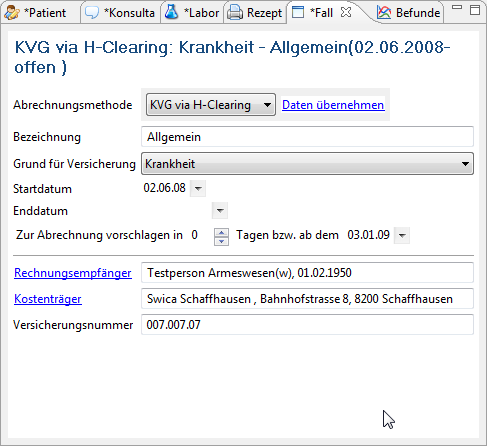
\includegraphics[width=0.8\textwidth]{images/falldetail}\\
  \caption{Fall-Detail}\label{fig:falldetail}
\end{figure}
Indiquez dans la boîte de choix en haut quel système de facturation doit être appliqué pour ce cas (cf aussi \ref{settings:abrechnungssystem} page \pageref{settings:abrechnungssystem}). En dessous il y a un espace où vous pouvez choisir librement une désignation pour le cas. Celui-ci ne sert qu'à vos propres informations, afin que
 vous puissiez mieux distinguer les différents cas du même patient.
La prochaine ligne, 'la raison pour l'assurance' est une indication qui apparaîtra sur les factures qui concernent le cas (si jamais le modèle de facturation contient un champ spécifique pour cela).

La\textbf{date de départ } est généralement la date de la première consultation, ou en cas d'accident, la date de l'accident. La  \textbf{date finale } désigne la date quand le cas est terminé. Un cas qui a une date de fin, est marqué comme 'cas terminé' dans la liste des cas  (Fig. \ref{fig:faelle2}) . Le cas terminé ne permet plus de ajouter une consultation de plus. 
Généralement, un cas ne devrait être terminé que s'il s'agit d'un accident qui est terminé, ou si le patient change d'assureur et si les données de facturation changent pour cette raison.

La prochaine ligne, destinataires de la facture, est impérative, afin qu'une facture puisse effectivement être fournie. Cela doit être un contact déjà existant (p. ex. le patient lui-même).

\medskip
Toutes les autres lignes seront selon le choix du système de facturation différentes. Souvent il y existera aussi une ligne 'répondant des coûts' \footnote{Remarque importante : Pour le \textbf{système Tarmed } (Suisse): Si le destinataire de la facture et le répondant des coûts est identique, une facture Tiers-Payant est fourni, autrement une facture Tiers-garant . Veillez ainsi à ce que ces deux lignes soient correctes (Pour des cas LAA les assureurs d'accident doivent être les destinataires de la facture et en même temps répondants des coûts tandis qu'avec les cas LAMAL le patient est destinataires de la facture dans les cantons Tiers garants et la caisse de maladie est répondant des coûts.)}.

\clearpage

\subsection{Diagnostics}
\label{view:diagnosen} \index{Diagnostics}
Cette 'View' (Fig. \ref{fig:diagnosen}) sert à choisir des diagnostics et de les assigner aux consultations respectives. \begin{wrapfigure}{l}{7cm}
    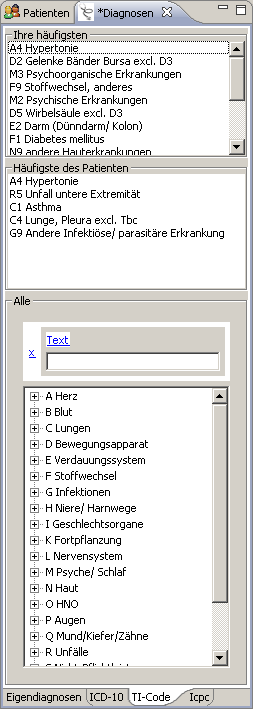
\includegraphics[width=6.5cm]{images/diagnosenview}
    \label{fig:diagnosen}
    \caption{Diagnosen-Auswahl}
\end{wrapfigure}
Vous voyez vers le bas une série d'onglets qui correspondent aux Plugins de code de diagnostic installés. (comme standard : Code tessinois, CIM-10, et CISP-2). Pour choisir un diagnostic vous choisissez d'abord entre ces onglets le système de codification correspondant et ensuite le code.
Le choix peut avoir lieu par 'Drag and Drop' ou par double-clic .
Vous voyez pour chaque système de codification, une fenêtre divisée en trois : Dans le secteur supérieur se trouvent vos diagnostics les plus fréquemment utilisés (c.-à-d. de l'utilisateur actuellement connecté) ; dans la partie moyenne se trouvent les diagnostics qui ont jusqu'ici le plus fréquemment été utilisés pour le patient en question et dans la partie inférieure se trouve la systématique entière du système de codification choisi.



\medskip

De cette façon vous avez toujours accès aux codes des diagnostics les plus fréquemment utilisés et vous n'auriez que rarement à fouiller la systématique entière.

